\subsection{From RAG to Agent}
% 

\begin{figure*}[t]
    \centering
    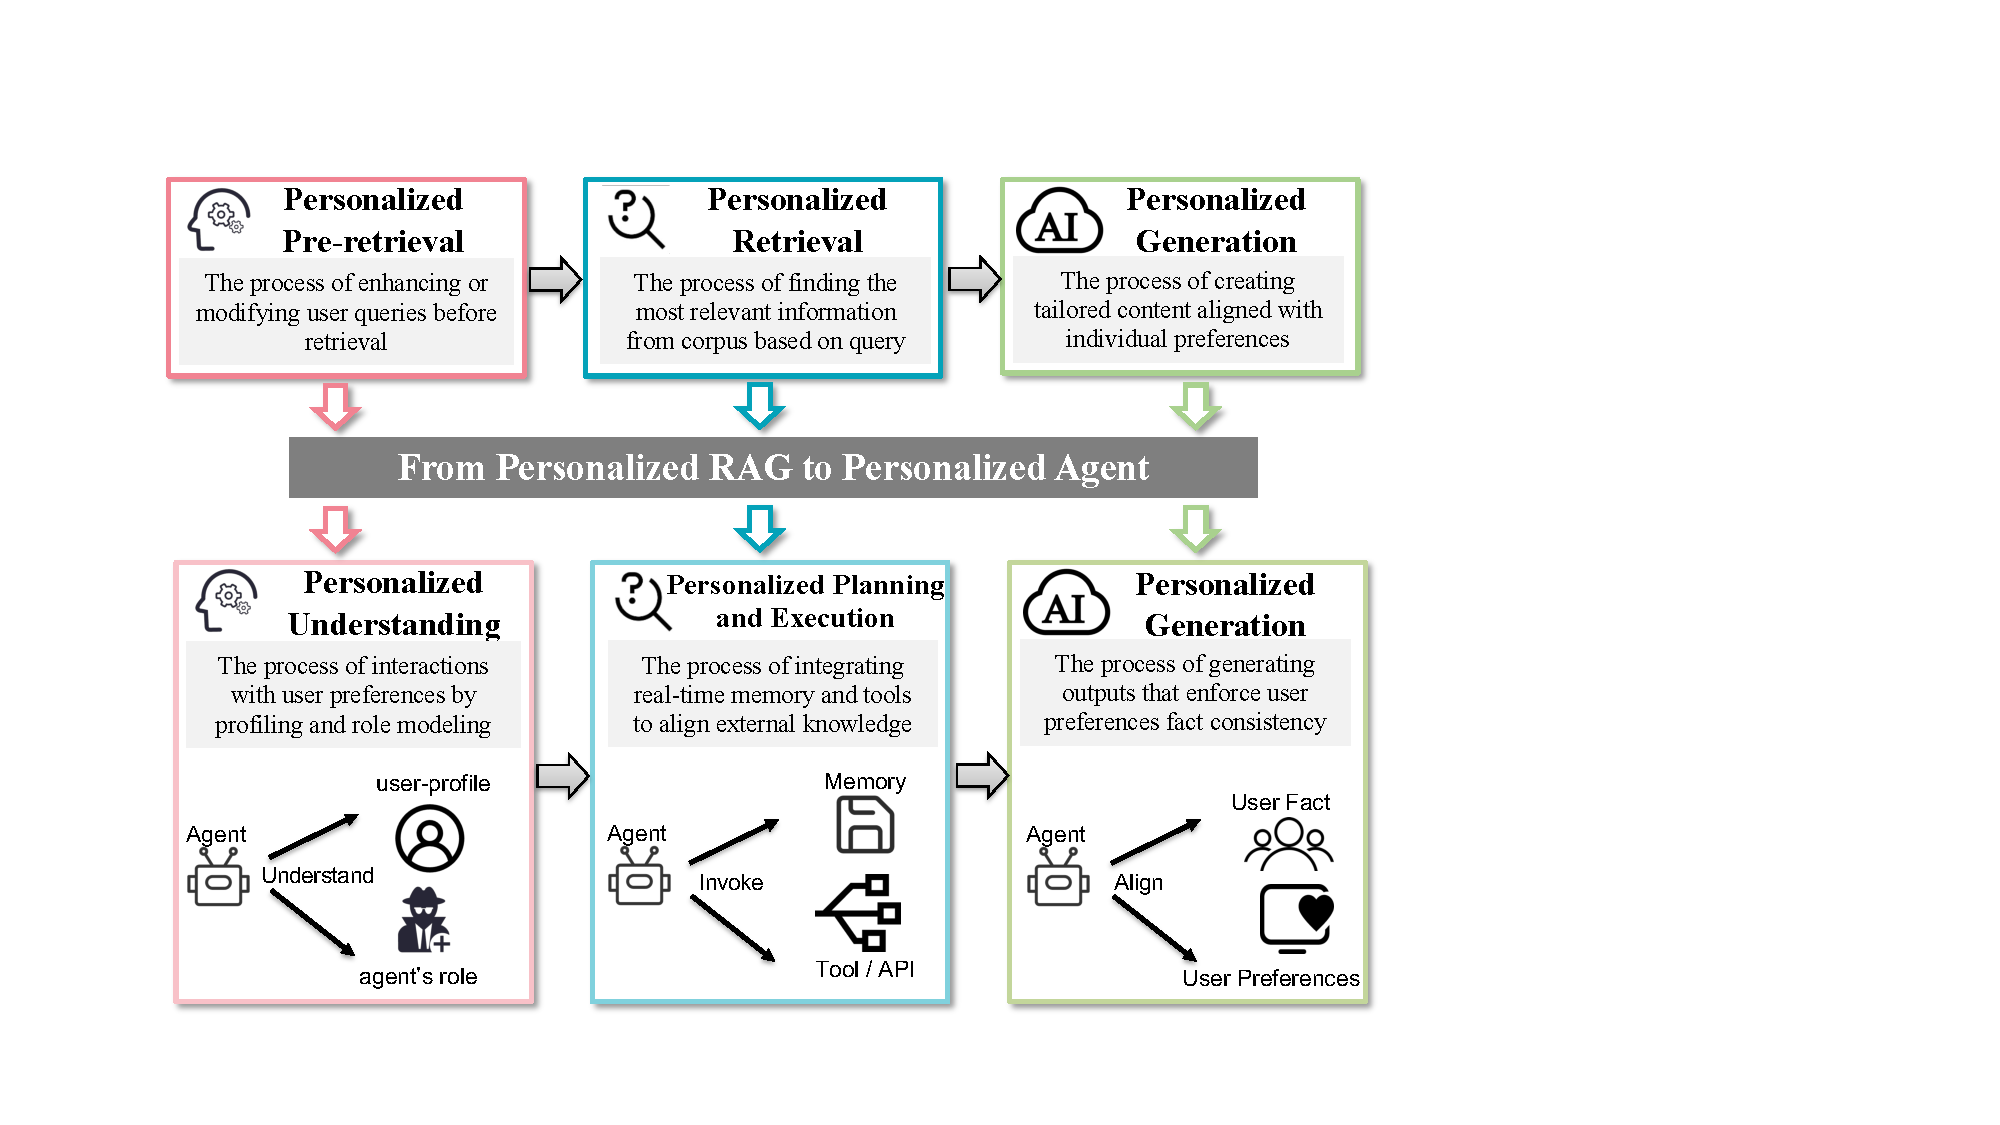
\includegraphics[width=\linewidth]{figures/PRAG_agent.pdf}
    \caption{Overview of transition from personalized RAG to personalized agent.}
    \label{fig:Agent}
\end{figure*}


\subsubsection{\textbf{Definition}}
A personalized LLM-based agent is a system designed to dynamically incorporate user context, memory, and external tools or APIs to support highly personalized and goal-oriented interactions \cite{xi2025rise,huang2024understanding,chen2024persona}, and solve problems in a goal-oriented manner \cite{li2024personal,singh2025agentic}.
From the previously introduced stages of RAG, we observe that the evolution of personalized RAG reveals a structural convergence with agent architectures. We analyze them from three key perspectives: 
\begin{itemize}[leftmargin=*]
\item \textbf{Personalized Understanding}: This phase within the agent parallels the query understanding and rewriting process of RAG as outlined in Section \ref{sec:Pre-retrieval}. However, it extends beyond static semantic parsing by incorporating dynamic user profiling \cite{wang2023rolellm} and role modeling \cite{shao2023character}. This integration enables the agent to dynamically align interactions with implicit user preferences, facilitating personalized responses and task-specific adaptations \cite{ran2024capturing}.
%
\item \textbf{Personalized Planning and Execution}: This phase in agents mirrors RAG's retrieval process in Section \ref{sec:Retrieval} yet it advances beyond static document retrieval by incorporating real-time memory management \cite{park2023generative} and sophisticated tool and API calling \cite{wangvoyager}. This approach ensures the dynamic alignment of external knowledge with personalized constraints, such as integrating medical history in healthcare agents \cite{abbasian2023conversational}, to deliver context-aware and user-specific outcomes. %\yc{can use the structure of this paragraph to refine the first and third perspectives.}
%
\item \textbf{Personalized Generation}: This phase in agents mirrors RAG's generative process in Section \ref{sec:Generation} but transcends static template-based generation by integrating user preference and fact alignment. Agents dynamically enforce user preferences and ensure fact consistency through role-specific mechanisms (\eg social adaptability in conversational agents \cite{abbasian2023conversational}), enabling outputs to evolve in harmony with personalized and situational constraints rather than relying solely on predefined generative frameworks.

\end{itemize}
 In general we frame agent architectures as ``\textbf{personalized RAG++}'', where persistent memory \cite{wang2024crafting} replaces static indexes, and tool APIs \cite{cai2025large} serve as dynamic knowledge connectors, enabling complicated, human-aligned interactions beyond one-shot retrieval, as shown in Figure \ref{fig:Agent}. This progression highlights that as RAG systems incorporate deeper personalization—requiring user-state tracking, adaptive tool usage, and context-aware generation, they inherently adopt agent-like capabilities.

\subsubsection{\textbf{Personalized Understanding}}
Personalized understanding refers to an agent’s ability to accurately interpret user inputs by integrating user intent recognition and contextual analysis. This process ensures interactions that are both meaningful and contextually appropriate. The rationale behind this classification lies in its capacity to address three core aspects of understanding: recognizing user intent, analyzing context, and leveraging user profiles. Each of these aspects plays a distinct role in improving the agent's performance. %\yc{emphasize the rationale of these three classification, what are the different impacts on query/user understanding}

\paragraph{\textbf{\textit{{(1). User-profile Understanding.}}}}
In user-profile understanding, an agent's personalized ability primarily depends on its capacity to accurately model and understand the user's preferences, context, and intentions. \citet{xu2024penetrative} proposes a framework in which LLMs are designed to understand the physical world, thereby facilitating a deeper connection between the agent and its environment, which is essential for accurate task execution. \citet{abbasian2023conversational} further expands this understanding by emphasizing the importance of personalization in health agents, where the user’s profile directly influences the behavior and decisions of the agent. This user understanding is foundational to ensuring that the AI agent performs tasks in a way that aligns with individual user needs.

\paragraph{\textbf{\textit{{(2). Role Understanding.}}}}
In agent's role understanding, the role of the agent within these environments is also crucial. Recent studies focus on enhancing role-playing capabilities within LLMs. \citet{wang2023rolellm} introduce RoleLLM, a benchmark that aims to elicit and refine the role-playing abilities of LLMs, demonstrating how role understanding influences agent performance in conversational tasks. Similarly, \citet{shao2023character} present Character-LLM, a trainable agent framework for role-playing, which tailors its responses based on predefined roles. \citet{wang2023incharacter} introduce a method for evaluating personality fidelity in role-playing agents through psychological interviews, aiming to enhance the realism and consistency of AI-driven characters. This role understanding allows for more contextually appropriate interactions, increasing the relevance and utility of AI agents across various applications. %\yc{what is the relation with user-profile, and user/query understanding}

\paragraph{\textbf{\textit{{(3). User-role Joint Understanding.}}}}
In agent's user-role joint understanding, the intersection of user and role understanding is explored through frameworks that evaluate and enhance the social and personality aspects of LLMs. SocialBench \citet{chen2024socialbench} provides a sociality evaluation framework for role-playing agents. \citet{dai2024mmrole}, and \cite{ran2024capturing} extend this by incorporating multi-modal data and personality-indicative information, respectively, which allows agents to better adapt to both user and role understanding in dynamic environments. Furthermore, \citet{wang2023enabling} offers a perspective on how role and environment understanding can improve user experience. \citet{tu2024charactereval} contribute by providing a benchmark specifically for evaluating role-playing agents in the Chinese context, adding a cultural dimension to role understanding. Finally, Neeko \cite{yu2024neeko} further advances role-based interactions.


\subsubsection{\textbf{Personalized Planning and Execution}}
Personalized planning and execution refer to the process of designing and implementing strategies or actions that are specifically tailored to an individual’s unique context, and goals \cite{huang2022language,zhangbootstrap,park2023generative,singh2024personal}. It requires agents to dynamically integrate long-term memory, real-time reasoning, and external tool utilization \cite{hong2023metagpt,zheng2023agents,hongru2023large}, as demonstrated in healthcare decision support \cite{abbasian2023conversational} and travel planning scenarios \cite{cai2025large}. We analyze two fundamental components that enable this personalization in the following.

\paragraph{\textbf{\textit{{(1). Memory Management.}}}}
Effective memory systems allow agents to integrate users' historical preferences, behavioral patterns, and contextual habits, enhancing their ability to make planning and tailor interactions to user-specific needs \cite{wangvoyager,cai2025large,wangmemoryllm}. The EMG-RAG framework \cite{wang2024crafting} combines editable memory graphs with retrieval-augmented generation to maintain dynamic user profiles, while \citet{park2023generative} implements memory streams and periodic reflection mechanisms to simulate human-like behavior. In healthcare applications, \citet{abbasian2023conversational} integrates multimodal user data through specialized memory modules to optimize treatment recommendations. For recommendation systems, RecAgent \cite{wang2023user} employs hierarchical memory structures to model user interaction patterns across multiple domains. Recent advances like TravelPlanner+ \cite{singh2024personal} demonstrate how memory-augmented LLMs achieve higher relevance in personalized itinerary generation compared to generic planners. %\yc{current description seems to have no relation with planning}

\paragraph{\textbf{\textit{{(2). Tool and API Calling.}}}}
The integration of external tools expands agents' capabilities beyond pure linguistic reasoning, enabling agents to interact with users and perform personalized tasks \cite{cai2025large,zhangbootstrap,xu2024penetrative,wangvoyager,wang2023enabling}. For instance, VOYAGER \cite{wangvoyager} establishes a paradigm for lifelong skill acquisition through automatic API curriculum learning and skill library construction. In robotics, \citet{zhangbootstrap} develops a bootstrapping framework where LLMs guide robots in tool-mediated skill discovery, enabling a high success rate in novel object manipulation tasks. The PUMA framework \cite{cai2025large} demonstrates how personalized web agents can achieve performance gains in e-commerce tasks through adaptive API orchestration. For mobile interaction, \citet{wang2023enabling} implements few-shot tool learning to handle diverse UI operations with minimal training data. These approaches highlight the importance of tool grounding mechanisms \cite{huang2022language} that translate linguistic plans into executable API sequences while maintaining personalization constraints.

This synthesis highlights that modern agent systems achieve enhanced personalization through two primary strategies: 1) Memory-augmented architectures, which leverage editable memory graphs \cite{wang2024crafting}, reflection mechanisms \cite{park2023generative}, and hierarchical memory structures \cite{wang2023user} to dynamically adapt to user preferences across various domains; and 2) Tool and API integration, which expand agent capabilities by balancing generalization  with specialization. Future work may explore improving the contextual relevance and adaptability of memory systems while optimizing real-time tool interaction for seamless task execution.



\subsubsection{\textbf{Personalized Generation}}
Based on the foundation of personalized planning and execution mechanisms, which enable agents to adapt strategies to user-specific contexts \cite{huang2022language,zhangbootstrap}, the next critical concern lies in personalized generation. This capability ensures that generated outputs not only align with factual correctness but also resonate with users' unique preferences, personality traits, and situational needs. Personalized generation bridges the gap between adaptive reasoning and human-aligned outcomes, allowing agents to produce contextually relevant and emotionally appropriate responses.

\paragraph{\textbf{\textit{{(1). Alignment with User Fact.}}}}
Alignment with User Fact emphasizes the accuracy, consistency, and factual grounding of personalized responses, ensuring they remain trustworthy across diverse user interactions. This is particularly challenging in personalized agents, where maintaining character authenticity while avoiding hallucinations requires balancing creativity with factual adherence.
Recent advances address these challenges through improved training frameworks and evaluation metrics. For instance, Character-LLM \cite{shao2023character} integrates memory-augmented architectures to reduce hallucinations while preserving character-specific traits. \citet{wang2024investigating} investigate quantization effects on personality consistency in edge-deployed agents and stabilize outputs under computational constraints. \citet{dai2024mmrole} ensures multimodal consistency (text-image) in role-playing. These works highlight the importance of architectural innovations and rigorous evaluation in achieving reliability.

\paragraph{\textbf{\textit{{(2). Alignment with User Preferences.}}}}
Alignment with user preferences ensures that generated outputs reflect individualized personalities, values, and interaction styles. This requires agents to dynamically interpret implicit user cues and adapt responses accordingly.
\citet{wang2023rolellm} benchmarks role-specific alignment. \citet{ran2024capturing} improves personality fidelity via psychological scale datasets. \citet{wang2023incharacter} quantifies alignment via psychological interviews. \citet{chen2024socialbench} evaluates social adaptability in conversations.

\subsubsection{\textbf{Discussion}}
The architectural evolution from RAG to personalized agents introduces significant advancements in human-AI interaction but also surfaces critical challenges that warrant further investigation.

\textbf{Personalized Understanding}, while enabling interpretation of user intent and context, faces limitations in real-time adaptability and generalization. Current approaches like RoleLLM \cite{wang2023rolellm} and Character-LLM \cite{shao2023character} demonstrate robust role-specific comprehension but struggle with dynamic user state tracking, particularly when handling evolving preferences or multi-session interactions. Furthermore, cultural specificity in benchmarks like CharacterEval \cite{tu2024charactereval} reveals gaps in global applicability, as agents trained on region-specific data often fail to generalize across diverse sociocultural contexts. Future work could explore hybrid architectures that combine continuous learning mechanisms with privacy-preserving federated learning to address these adaptability constraints while maintaining user trust.

\textbf{Personalized Planning and Execution}, achieves remarkable task specialization through memory management and tool integration, yet suffers from scalability issues in complex environments. While frameworks like EMG-RAG \cite{wang2024crafting} and VOYAGER \cite{wangvoyager} effectively manage user-specific constraints, their reliance on predefined API taxonomies limits emergent tool discovery in novel scenarios. The "cold-start" problem persists in domains requiring rapid skill acquisition, as seen in healthcare applications \cite{abbasian2023conversational}, where delayed API responses can compromise decision-making efficacy. A promising direction involves developing meta-reasoning architectures that dynamically prioritize memory recall versus tool invocation based on situational urgency and confidence thresholds.

\textbf{Personalized Generation} balances factual accuracy with preference alignment but risks over-fitting, where excessive finetuning to user profiles may reinforce cognitive biases. Techniques address surface-level alignment but lack mechanisms for ethical boundary detection. For instance, agents might inadvertently propagate harmful stereotypes when mirroring user preferences without critical oversight. Future systems could integrate value-aligned reinforcement learning with human-in-the-loop validation to preserve authenticity while preventing detrimental customization.

